\chapter{Человеко-машинный интерфейс}

В рамках данной работы человеко-машинный интерфейс представлен в виде пользовательских окон управления в Unity Editor, а также в виде онлайн-ресурса посвящённого обучению и модификации описываемой работы.

\label{cha:ch_3}
При создании окон управления не были использованы ни синглтон заготовки, ни написанный DI контейнер ввиду особенностей распределения времени выполнения  у \textit{Unity} -- пространство имен, взаимодействующее с классами, которые регламентируют внешний вид и поведение пользовательских окон, изолировано от других пространств, что делает невозможным использование DI и других вспомогательных структур. 

\section{Окно управления записью и проигрыванием}
Данное окно (см. рис. \ref{recorderUI}) состоит из трёх секций: указание текущей реализации проигрывателя, состояние проигрывателя и элементы управления проигрыванием и записью.

\begin{figure}[h]
	\centering
	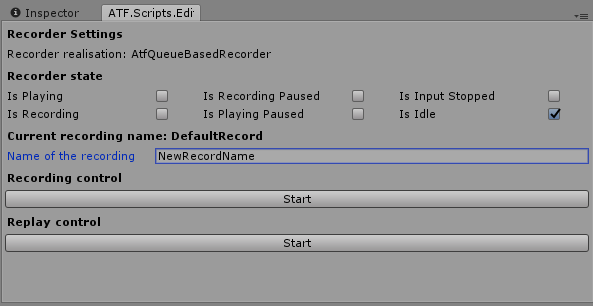
\includegraphics[width=0.7\linewidth]{recorder.PNG}
	\caption{Editor UI для проигрывателя}
	\label{recorderUI}
\end{figure}

В процесс управления записью входит:
\begin{itemize}
	\item
	просмотр текущего состояния проигрывателя по чекбоксам состояния на рис.\ref{recorderUI};
	\item
	определение имени записи, которую нужно проиграть или под которое нужно записать поток действий;
	\item
	непосредственно сами кнопки управления записью -- Start, Stop, Play, Continue;
	\item
	аналогичные кнопки управления проигрыванием -- Start, Stop, Play, Continue.
\end{itemize}
Для того чтобы проиграть выбранную запись, необходимо сначала вписать нужное имя в поле \textit{Name of the recording} или же просто щёлкнуть правой кнопкой мыши по записи в активной зоне окна управления хранилищем.

\section{Окно управления хранилища действий}
Окно управления хранилищем (см. рис. \ref{storageUI}) также состоит из трёх секций -- информация о реализации, секции управления сохранением и загрузкой, а также зоны иллюстрации текущего состояния хранилища.

\begin{figure}[h]
	\centering
	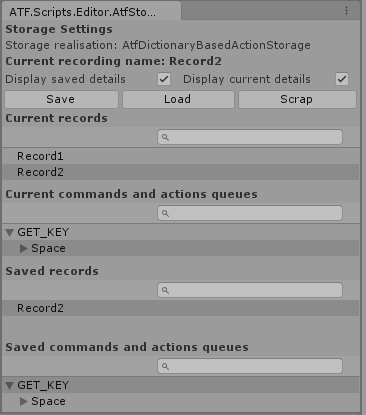
\includegraphics[width=0.7\linewidth]{storage.PNG}
	\caption{Editor UI для хранилища действий}
	\label{storageUI}
\end{figure}

В процесс управления хранилищем входит:
\begin{itemize}
	\item
	просмотр текущей записи хранилища;
	\item
	определение имени записи, которую нужно загрузить или сохранить; 
	\item
	непосредственно сами кнопки управления сохранением -- Save, Load, Scrap (удалить);
	\item
	загрузка в активную зону записей из реестра (Окна: Current records, Current commands and actions queues).
\end{itemize}
Зоны иллюстрации хранилища делятся на активную и пассивную. Активная зона хранит в себе те записи, которые находятся сейчас непосредственно в оперативной памяти, пассивная же зона хранит в себе записи, которые были сохранены на внешнем накопителе или реестре.

\section{Окно управления интеграцией}

Окно управления интеграцией (см. рис. \ref{integratorUI}) состоит из трёх секций -- информация об используемой реализации, секция добавления и удаления путей к файлам исходного кода и секция с отображением выбранных файлов и кнопками управления.

\begin{figure}[h]
	\centering
	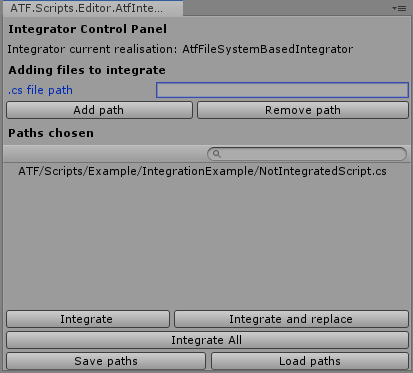
\includegraphics[width=0.7\linewidth]{integrator.PNG}
	\caption{Editor UI для управления интеграцией}
	\label{integratorUI}
\end{figure}

Так как система интеграции поддерживает два режима работы: автоматический и полуавтоматический, при проектировании данного окна было решено выделить отдельные кнопки для обоих режимов:
\begin{itemize}
	\item
	Кнопки \textit{Integrate} и \textit{Integrate and replace} отвечают за полуавтоматический режим и воздействуют на представленные в третьей секции конкретные файлы исходного кода.
	\item
	Кнопка \textit{Integrate All} отвечает за использование автоматического режима.
\end{itemize}

Кнопки \textit{Save paths} и \textit{Load paths} отвечают за сохранение и загрузку представленных в третьей секции файлов исходного кода. Для облегчения работы с файлами, вместо конкретных файлов во второй секции было решено использовать пути файлов.

\section{Онлайн-документация}
Для лучшего понимания функционала разработанной группы ассетов была создана онлайн-документация \cite{atf_docs}. Данный ресурс содержит в себе учебный материал не только для обучения пользованием ассетами, но и информацию о каждом интерфейсе основной системы и учебный материал, где рассказывается о том, как можно модифицировать разработанные ассеты, а также создавать новые.

В качестве платформы для создания онлайн-документации было решено использовать ReadTheDocs.org с генератором документации Sphinx (см. рис. \ref{online_docs}). Критерием к выбору платформы и генератора служила возможность бесплатного хостинга ресурса с адекватным на мнение автора именем хоста, лёгкость языка шаблонизатора у генератора, а также высокий уровень репутации ресурса.

Это было необходимо, чтобы не отпугнуть потенциального контрибьютора от изучения документации.

\begin{figure}[H]
	\centering
	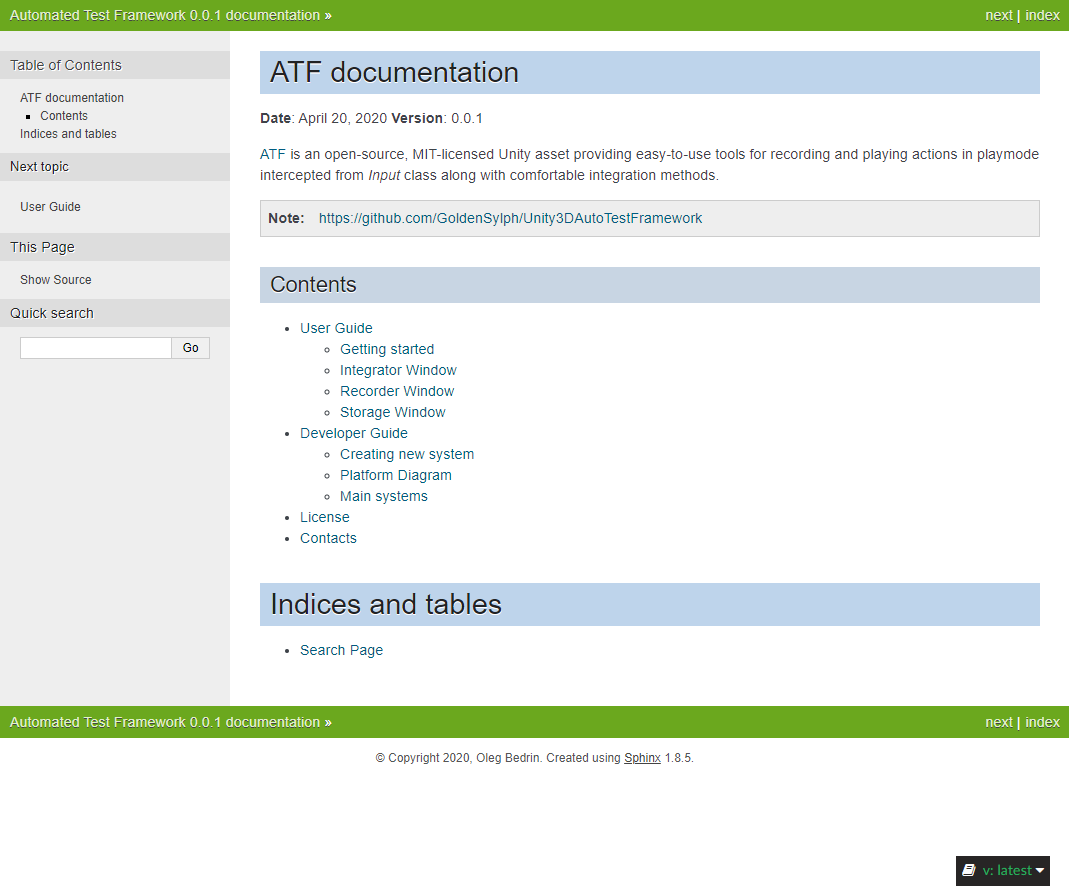
\includegraphics[width=\linewidth]{online_docs.png}
	\caption{Главная страничка онлайн-документации}
	\label{online_docs}
\end{figure}

В дополнение к созданной онлайн-документации была добавлена возможность быстрого поиска по статьям представленным в ней.

